\documentclass[12pt]{report}

% some macros
% Here, you can define your own macros. Some examples are given below.

\newcommand{\R}[0]{\mathds{R}} % real numbers
\newcommand{\Z}[0]{\mathds{Z}} % integers
\newcommand{\N}[0]{\mathds{N}} % natural numbers
\newcommand{\C}[0]{\mathds{C}} % complex numbers
\newcommand{\bm}[1]{{\boldsymbol{{#1}}}} % vector
\newcommand{\mat}[1]{{\boldsymbol{{#1}}}} % matrix

\newcommand{\E}[1]{\mathbb{E}_{#1}} % Expectation
\newcommand{\Pd}[1]{\mathbb{P}_{#1}} % Probability Distribution

%%%%%%%%%%%%%%%%%%%%%%%%%%%%%%%%%%%%%%%%%
% University Assignment Title Page 
% LaTeX Template
% Version 1.0 (27/12/12)
%
% This template has been downloaded from:
%%%%%%%%%%%%%%%%%%%%%%%%%%%%%%%%%%%%%%%%%
%----------------------------------------------------------------------------------------
%	PACKAGES AND OTHER DOCUMENT CONFIGURATIONS
%----------------------------------------------------------------------------------------

\usepackage[nottoc,notlot,notlof]{tocbibind}
\usepackage[T1]{fontenc}
%\usepackage{hyperref}
\usepackage{indentfirst}
\usepackage{amsmath}
\usepackage{amssymb}
\usepackage{graphicx}
\usepackage{subcaption}
\usepackage{geometry}
 \geometry
 {
     a4paper,
     left=25mm,
     right=25mm,
     top=30mm,
     bottom=30mm,
 }

% \usepackage[a4paper,hmargin=2.8cm,vmargin=2.0cm,includeheadfoot]{geometry}
\usepackage{textpos}
\usepackage{natbib} % for bibliography
%\usepackage{tabularx,longtable,multirow,subfigure,caption}
\usepackage{fncylab} %formatting of labels
\usepackage{fancyhdr} % page layout
\usepackage{url} % URLs
\usepackage[english]{babel}
%\usepackage{dsfont}
\usepackage{epstopdf}
\usepackage{backref} % needed for citations
\usepackage{array}
\usepackage{latexsym}
\usepackage[pdftex,pagebackref,hypertexnames=false,colorlinks]{hyperref} % provide links in pdf
 
\hypersetup{pdftitle={},
  pdfsubject={}, 
  pdfauthor={},
  pdfkeywords={}, 
  pdfstartview=FitH,
  pdfpagemode={UseOutlines},% None, FullScreen, UseOutlines
  bookmarksnumbered=true, bookmarksopen=true, colorlinks,
    citecolor=black,%
    filecolor=black,%
    linkcolor=black,%
    urlcolor=black}
 
\usepackage[all]{hypcap}
\frenchspacing

\DeclareMathOperator{\tr}{tr}

\begin{document}

\chapter{Literature Review}

TODO
Add introduction to lit review

\section{Current Lip Reading Models and Datasets}

%This section shall discuss current lip reading models built with deep learning techniques and the availability of both 2D and 3D temporal datasets which lip reading models can currently be trained on.
In recent years the problem of Lip Reading has seen huge advances due to the availability of new datasets and the use of Deep Learning models.
This section shall discuss the progresses which have already been made in this field and the datasets publicly available on which to train such models.
Current lip reading models, to the best of the author's knowledge, all make use of 2D temporal data such as videos by evaluating the frames of the video, using this information to make a prediction of the word, or words, which were spoken in the sequence.
Video data is convenient as it is widely available and relatively straightforward to obtain and process.

However in reality, humans who are able to lip read also have access to three dimensional data due to our depth perception, which is not well represented in 2D video frames; thus is can be hypothesised that some information captured by 3D temporal scans of speaking subjects can also be used for speech prediction.
Unlike 2D temporal data, 3D temporal data (3D video), requires multiple cameras to record simultaneously, which in turn requires synchronisation between the cameras, increasing the complexity of the system beyond simply having multiple cameras.
The data must then be processed to produce the final product, whether this is in the form of video with depth information or more complex 3D scans \cite{Li2017}.

\subsection{Datasets}
There currently exists multiple labelled video datasets which can be used for traditional lip reading; here 'traditional' refers to using 2D temporal data.
Datasets such as GRID \cite{Cooke2006}, LRW \cite{Chung2016}, LRS \cite{Chung2017} and LSVSR \cite{Shillingford2018} have been constructed by compiling the video data from various sources, each with an increasing vocabulary and dataset size.

\subsubsection{Controlled Conditions Datasets}
The GRID dataset was released in 2006 \cite{Cooke2006} and contains 34,000 samples from 34 speakers, each with 1000 sentences.
The corpus uses sentences with a fixed grammar: 
<command:4>, <colour:4>, <preposition:4>, <letter:25>, <number:10>, <adverb:4>, with a total vocabulary of 51 words.
Aside from the restricted vocabulary size in comparison to more recent datasets, the primary limiting factor of the GRID dataset is that all data was captured directly for the use of the dataset and so, models trained on this dataset have learnt on controlled conditions, something not found in the desired wider applications of lip reading.

\subsubsection{In The Wild Datasets}
To build larger datasets, the following are commonly built with "in the wild" data, meaning that the videos have not been captured with the intention of being used for this dataset.
Variations in lighting, angles, speakers and a wide vocabulary are common, this does however make the datasets more challenging to learn from, but the models are no longer as bias to controlled conditions.

LRW and LRS are both comprised of content from BBC broadcasts \cite{Chung2016, Chung2017} allowing for a far larger corpus size of over 500 words for LRW and over 6000 words for LRS.
Both of datasets are captured and processed with the same pipeline summarised as follows. 
Firstly, as the subtitles are not aligned to the video on the broadcasts, optical chapter recognition is used to obtain the text being spoken in the video clips, the audio and text are then aligned per frame using the HTK toolkit \cite{Woodland1995}. 
A histogram of oriented gradients based (HOG-based) detection algorithm \cite{King2009} is used for face detection for cropping the frames to the subjects head followed by facial landmarks for mouth localisation and speaker identification in order to crop the video frames the the point of interest.

LSVSR is a dataset published by DeepMind and Google which makes use of the huge amount of videos on YouTube \cite{Shillingford2018}, resulting in a total length of 3886 hours of training data.
The dataset is far larger than LRS, but aligns phonemes to frames, as opposed to words or characters.
The pre-processing steps are similar as in LRW and LRS; alignment is performed with the algorithm laid out in previous work by DeepMind \cite{Liao2013}, faces are tracked to ensure the speaker is visible in frame.

\subsubsection{3D Datasets} \label{3D Datasets}
To the best of the author's knowledge, there are currently two datasets with 3D temporal data which are appropriate for training lip reading models.
The first of which is LRW-3D \cite{Tzirakis2019} which has been captured from four subjects, two native English speakers and two non-native to increase variability in the dataset.
The subjects have been captured speaking the corpus used in the LRW dataset \cite{Chung2016}, a vocabulary of 500 words.
The resulting dataset comprises of 660 seconds of 3D meshes and audio per subject.
The dataset is not comprised of full sentences but would be appropriate for word-level lip reading, however a total duration of 660 seconds is likely to be too short for a deep learning model to train effectively.

The second is the VOCASET \cite{Cudeiro2019}, an unlabelled dataset captured from 6 male and 6 female subjects.
Each subject was recorded speaking 40 sequences, each ranging from 3 to 5 seconds, resulting in a total time of 30 minutes.
The recorded 3D meshes are registered to the FLAME model \cite{Li2017}, a statistical 3D facial mesh with around 5000 vertices.
Unlike the LRW-3D dataset, the sequences are grammatically correct sentences, chosen to maximise phonetic diversity.
This makes the VOCASET appropriate for creating a model for sentence-level lip reading, similarly to LRW-3D, 30 minutes of training data is likely to be a limiting factor when training a deep learning model.

It should be noted that neither of these datasets were captured for the purpose of lip reading, but for synthesising realistic statistical facial models driven from an audio input, and thus the transcriptions and frames are not aligned.
This alignment would have to be performed to the datasets before using the data to train lip reading models.
In order to achieve this automatic speech recognition (ASR) systems such as DeepSpeech \cite{Hannun2014} could be used to solve this problem.

\subsection{Lip Reading Models}
Chung et al \cite{Chung2016} used a convolutional model based on the VGG-M architecture which produced character level distributions with the LRW dataset, these distributions are then processed by a language model for text prediction.

The LipNet model \cite{Assael2016} was produced to be able to predict sentence-level lip reading of varied length, while previous work by \cite{Chung2016} predicted on a word level.
The model used spatiotemporal convolutions to process multiple frames of video at once followed by a recurrent layer using Gated Recurrent Units (GRU) \cite{Cho2014}.
The model used the GRID dataset \cite{Cooke2006} in which all subjects are recorded under consistent conditions of good lighting and fixed angles.
LipNet achieved the state of the art performance on the GRID dataset by using an model with increased complexity by incorporating 3D convolution and recurrent units.

As the LRW dataset could not be used to train a model such as LipNet for sentence-level lip reading, but the GRID dataset had limitations in the number of subjects and vocabulary, Chung et al created the LRS dataset \cite{Chung2017}.
The model presented was trained on both audio and video and made capable of taking either or both as the model inputs.
To prevent the model from being dependent on a single input source, the inputs are systematically distorted or removed.
The video input is passed through convolutional layers, followed by LSTM layers, while the audio is converted to Mel-frequency cepstral coefficients (MFCC), then input to LSTM layers.
The two are combined with then attention mechanism and further LSTM layers and an output fully connected layer with softmax activation for character distributions.
The model also makes use of curriculum learning by initially training the model on short sequences of single words.
The length of training sequences are increased throughout training.
It is stated by \cite{Chung2017} that this accelerates training and reduces overfitting.

In 2018 DeepMind published their V2P model \cite{Shillingford2018} along with the LSVSR dataset which is larger than all previous datasets, containing 3886 hours of training data.
The model follows a similar architecture to LipNet \cite{Assael2016} but with an increased number of convolutional layers and LSTM layers rather than GRUs.
It should be commented that due to the size of the model and dataset dictated the use of 64 GPUs for training to allow a batch size of 128.
Unlike previous models, the V2P model predicts phonemes as opposed to characters, these phonemes are then processed by a language model for word prediction as with previous models.

To the best of the author's knowledge, currently there do not exist any papers which have explored the use of 3D temporal datasets for the use with lip reading models. 
This is likely due to the shortage of 3D temporal data due to the difficulties in obtaining such data, on which such models could be trained on.

\section{Data Generation}
In order to construct a deep learning lip reading model capable of being trained on 3D temporal data, appropriate datasets must be established.
Current datasets have been captured directly \cite{Tzirakis2019, Cudeiro2019} with the use of multi-camera capture rigs under controlled situations.
The total duration of both of these datasets is very short in comparison to the video datasets such as LRW, LRS and LSVSR, which is a limiting factor as to the models which could be trained using them.

As the models also use different mesh models to represent the data that has been captured this also prevents the two datasets being joined directly.
Unlike video data, there currently lacks a large body of 3D video data which is publicly available, limiting the construction of 3D datasets to directly capturing more 3D scans with multi-camera capture rigs, similar to those used in \cite{Tzirakis2019, Cudeiro2019} and generating synthetic training data.

\subsection{Audio Driven Data Generation}
Karras et al proposed a method for generating 3D facial animation from audio with the use of a CNN architecture \cite{Karras2017a}.
The model is actor specific, but is only trained on 3-5 minutes of data of the actor.
Short range temporal features are first extracted from the audio by a formant analysis network.
This representation is then analysed by an articulation network which also accepts a learned emotional state of the speaker.
The output layer drives displacements from a neutral 3d mesh of the actor.

However, as the model by Karras et al. is not independent of the actor it cannot generalise to new subjects.
Tzirakis et al. propose a model which is independent of speaker and capture rig \cite{Tzirakis2019}.
As discussed in section \ref{3D Datasets}, a dataset was constructed of 3D speaking faces using the LRW dataset \cite{Chung2016} for the corpus.
This allowed Tzirakis et al. to create a model which can synthesise facial motion from audio from the LRW dataset.
The model used is similar to that used in \cite{Karras2017a}, firstly extracting short term temporal features from the input audio with a convolutional network followed by another convolutional network to analyse the extracted features.
Unlike the model used in \cite{Karras2017a}, the model used in \cite{Tzirakis2019} is trained to drive learnt blendshapes.
This reduces the number of output parameters of the model substantially in comparison to that used by Karras et al.

Similar to \cite{Tzirakis2019}, the VOCA model \cite{Cudeiro2019} synthesises video sequences of 3D models speaking given an audio input.
The VOCASET dataset discussed in section \ref{3D Datasets}, was captured with the intention of training this model to be independent of the speaker, hence a large range of speakers are used within the dataset.
The model is comprised of three sections: audio feature extraction, a feature encoder and a decoder to drive a template facial mesh from the FLAME model \cite{Li2017}.
The audio feature extraction makes use of the pre-trained Mozilla implementation of the DeepSpeech model, based on the paper by Hannun et al. \cite{Hannun2014}.
The DeepSpeech model takes audio as an input and returns the unnormalised log-probabilities for an alphabet of the 26 standard characters, a space, apostrophe and blank character for time slices in the audio input.
The encoder is a convolutional network which is conditioned on the speakers identity, such that the latent space of speaker styles can later be explored on new audio inputs.
Finally, the decoder is made up of a fully connected layer with a linear activation function is used to output the displacements of the 5023 vertices in the template face.

\subsection{Adversarial Trained Generative Methods}
A recent development in generating synthetic data samples is the use of generative adversarial networks \cite{Goodfellow2014}.
The concept behind generative adversarial networks (GANs) is two have two machine learning models; a generator and a discriminator.
The task of the generator is to produce samples from an unknown high order probability distribution which correctly resemble samples from the distribution defined by training data.
The generator achieves this by transforming a random sample from a known probability distribution, such as a Gaussian distribution as used in \cite{Goodfellow2014}, to a sample from the unknown distribution.
This is achieved by finding the function which maps between the two distributions.
The discriminator however, attempts to correctly learn to discriminate between the real and the fake generated samples.

\begin{equation} \label{eq:gans_loss}
    \min_{G} \max_{D} V(G, D) = \E{\bm{x} \sim p_{data}(\bm{x})} [\log D(\bm{x})]
                              + \E{\bm{z} \sim p_{z}(\bm{z})} [\log (1 - D(G(\bm{z})))]
\end{equation}
\quad

\noindent The original loss function (\ref{eq:gans_loss}) proposed by Ian Goodfellow forms a min-max game, where the loss of the generator is attempting to be minimised by having the discriminator label all the generated samples as real.
While the loss of the discriminator is maximised by correctly classifying real and fake samples.
The two networks are trained in an alternating fashion until the discriminator achieves an accuracy of 50\%, effectively making binary guesses between real and generated samples.

GANs however, are difficult to train for two main reasons.
Firstly, the equation (\ref{eq:gans_loss}) is challenging as it provides small gradients while generated samples are poor as discussed in \cite{Goodfellow2014}, making training difficult.
Progress in developing new loss functions is discussed in section \ref{Stability_to_GANs}
Secondly, early networks must also be balanced with a similar model capacity to prevent one from getting too much better than the other, preventing the other from improving.
Various architectural changes have improved this issue \cite{Radford2016, Zhang2018}, although it seems to be closely tied to the loss function being used \cite{Gulrajani2017}.

\subsubsection{Stability Improvements of GANs Networks} \label{Stability_to_GANs}
There have been a large number of papers presenting new techniques with differing levels of success and training stability, a small handful of key papers which provided large advances in the generative adversarial training model shall be discussed here.
A primary research focus around GANs has been in finding new loss functions on which to train the model to improve stability and performance.
The original loss function proposed in the original paper \cite{Goodfellow2014} identifies an issue with equation (\ref{eq:gans_loss}) in that the gradient back propagated to the generator when the generated samples are poor, is very low as shown in figure \ref{fig:Goodfellow_plot}.

\begin{figure}[h]
    \centering
        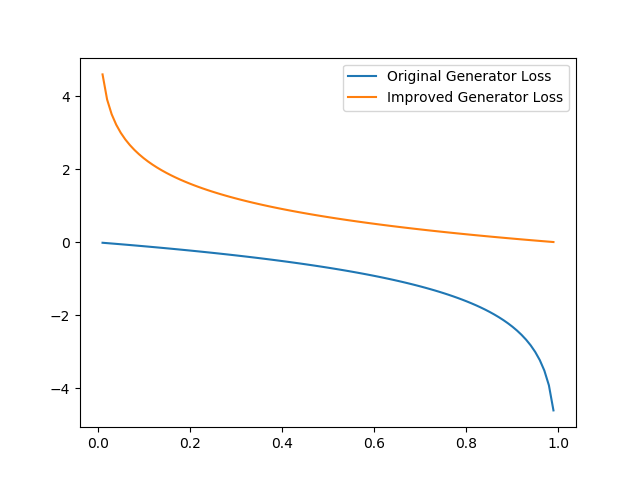
\includegraphics[width=0.8\textwidth]{figures/goodfellow_gen_losses.png}
    \caption{Goodfellow's Generator Loss Plots \cite{Goodfellow2014}}\label{fig:Goodfellow_plot}
\end{figure}
\quad

\noindent This in turn makes it very challenging to improve the performance of the generator.
The suggested improvement made in \cite{Goodfellow2014} is rather than to maximise the the number of generated samples which the discriminator incorrectly classifies, but to minimise the number of generator samples the discriminator correctly classifies, described in equation (\ref{eq:gans_loss2}).
Figure \ref{fig:Goodfellow_plot} shows how this results in the gradient propagated back to the generator is far larger when the generated samples are poor.

\begin{equation} \label{eq:gans_loss2}
    \min_{G} \max_{D} V(G, D) = \E{\bm{x} \sim p_{data}(\bm{x})} [\log D(\bm{x})]
                              - \E{\bm{z} \sim p_{z}(\bm{z})} [\log (D(G(\bm{z})))]
\end{equation}
\quad

Further stability improvements were proposed in \cite{Radford2016} which allowed deep convolutional generative adversarial networks (DCGANs) to be successfully trained for the first time.
Radford et al. proposed three main contributions.
Replace deterministic pooling layers with strided convolutions in both the generator and discriminator networks, allowing the networks to learn their own spatial upsampling and downsampling.
Remove all fully connected layers used on top of convolutional layers, resulting in a fully convolutional model.
Apply batch normalisation \cite{Ioffe2015} before the input of each layer.
This normalises the input to each unit to zero mean and unit variance.
This assists with training problems due to poor weight initialisation and allows gradients to flow through deeper networks more easily.
Radford et al. state this to be a critical improvement to allow generator networks to begin learning by preventing all samples from collapsing to a single point. 

In an attempt to stabilize the training of GANs models, the Wasserstein or 'Earth Mover Distance' loss function was proposed by Arjovsky et al. \cite{Arjovsky2017} shown in equation (\ref{eq:wgan}) where $\mathcal{D}$ is a set of 1-Lipschtiz functions.

\begin{equation} \label{eq:wgan}
    \min_{G} \max_{D \in \mathcal{D}} W(\Pd{r}, \Pd{g}) =
            \E{\bm{x} \sim \Pd{r}} [D(\bm{x})]
            -\E{\bm{\hat{x}} \sim \Pd{g}} [D(\hat{\bm{x}})]
\end{equation}
\quad

\noindent The WGAN model uses a critic as opposed to a discriminator, this is due to the fact that the discriminator is no longer a binary classifier, but being used to critique the real and generated samples. 
As the Wasserstein function is continuous and differentiable, the critic can be trained until optimality, and \cite{Arjovsky2017} argues that it should be.
As the critic is trained to optimality it does not saturate, but converges to a linear function.
This provides the generator with a gradient which is more reliable, resulting in the generator learning consistently.
The Wasserstein loss function has been shown to greatly improve training stability by providing consistent gradients throughout training and no longer requiring that the two networks have a balanced model capacity.

In order to use the Wasserstein distance as the loss for WGAN, the Lipschtiz condition must be enforced.
In the WGAN the model weights are clipped to enforce this constraint \cite{Arjovsky2017}, however this is stated to be a non-ideal method of achieving this constraint and calls for future work to be investigate more effective methods.
The use of gradient penalty is proposed in \cite{Gulrajani2017} in order to satisfy this condition more elegantly as described in equation (\ref{eq:wgan_gp}).

\begin{equation} \label{eq:wgan_gp}
    \min_{G} \max_{D \in \mathcal{D}} W(\Pd{r}, \Pd{g}) 
        = \E{\bm{\tilde{x}} \sim \Pd{g}} [D(\tilde{{\bm{x}}})]
        - \E{\bm{x} \sim \Pd{r}} [D(\bm{x})]
        + \lambda \E{\bm{\hat{x}} \sim \Pd{\bm{\hat{x}}}} 
            [(\| \nabla_{\bm{\hat{x}}} D(\bm{\hat{x}}) \| - 1)^2]
\end{equation}
\quad

\noindent Using the Wasserstein loss function with gradient penalty enforces the Lipschtiz condition and allows highly complex architectures to be trained successfully, including those with residual units \cite{Gulrajani2017}.

\subsubsection{Architectural Developments}
Mirza et al. showed that GANs could be conditioned on additional inputs to the generator network as the noise component \cite{Mirza2014}.
This has allowed facilitated other uses of GANs such as image to image translation for style transfer \cite{Zhu2017}.
Vougioukas et al. used a temporal model to generate a sequence of video frames given an image of a subject and an audio sequence of spoken text to synthesise the subject speaking \cite{Vougioukas2018}.
The model uses two discriminators, one to determine if individual frames are realistic images of the subject's face and a second which evaluates the sequence of video frames to determine if it is realistic.
The model uses temporal components to examine if the frames of video are consistent in time, preventing sudden jumps in facial position.

Other novel architectures include the progressively growing GAN model \cite{Karras2017b} which is able to generate highly realistic images of faces to a high resolution.
This is achieved by initially training a shallow model to produce 4x4 pixel images before increasing the depth of the network and training further at a higher resolution.
By forcing the model to firstly produce and examine low resolution images the model firstly has to be able to synthesise simple low level features effectively, such as facial shape which are common to all samples.
Once the model can produce these features a higher resolution is used, allowing it to learn more complex features, such as hair and eyes.

The attention mechanism \cite{Vaswani2017} has been shown to be usefully when applied to image data \cite{Xu2015} in order to capture relationships between spatially distant points.
As such points are further apart in the image, previously deeper convolutional models were required to allow a large enough receptive field to capture information on these two points.
Zhang et al. point out that this is a common issue with DCGANs \cite{Radford2016}, where generated samples fail to produce structural patterns, while they do exceedingly well at local textural patterns.
This is often seen in generated images of animals with realistic fur, but oddly shaped or an incorrect number of limbs.
The attention mechanism is applied to GANs \cite{Zhang2018} to allow for long range dependencies in the image to be modelled by convolutional models more effectively.

To the best of the author's knowledge, there currently exists no generative adversarial networks which aim to generate 3D facial models with speech audio as a conditional input.

\bibliographystyle{unsrt}
\bibliography{ref}
\end{document}
